% ARIN5203 Project Milestone Report
% Uses the CVPR style file if it is present (copy cvpr.sty / ieeenat_fullname.bst from the
% course template into this folder, or paste the body into the course Overleaf template).
% Without cvpr.sty it falls back to a plain two-column layout with similar margins.
\documentclass[10pt,twocolumn,letterpaper]{article}

\IfFileExists{cvpr.sty}{%
  \usepackage[pagenumbers]{cvpr}%
}{%
  \usepackage[letterpaper,top=1in,bottom=1in,left=0.75in,right=0.75in,columnsep=0.33in]{geometry}%
  \usepackage{times}%
}

\usepackage{graphicx}
\usepackage{amsmath}
\usepackage{amssymb}
\usepackage{booktabs}
\usepackage{multirow}
\usepackage[hidelinks]{hyperref}

\title{End-to-End Deep Portfolio Optimization with\\Risk- and Turnover-Aware Objectives\\[2pt]
\large ARIN5203 Project Milestone}

\author{Yiyang Lu (21383493) \qquad Jin Ziqi (21418846) \qquad Jingran Li (21327865)}

\begin{document}
\maketitle

%-------------------------------------------------------------------------
\section{Introduction}

End-to-end portfolio learning trains a network to output allocation weights directly and
scores it on portfolio performance, instead of forecasting returns and passing the forecasts to
an optimizer~\cite{zhang2020deep,kisiel2023portfolio}. We study one design choice in this
setting: the training objective. Starting from a small Transformer allocator, we add a variance
penalty and an L1 turnover penalty to a return objective and ask whether they lower
out-of-sample volatility and trading, whether the gains survive transaction costs, and what
return they cost relative to unregularized training and simple rules such as equal
weighting~\cite{demiguel2009optimal}. Our contribution is a controlled study of objectives, not a
new architecture.

Since the proposal we have built the full pipeline: a frozen six-ETF dataset, a weekly
cost-aware backtester shared by all strategies, three classical baselines, an LSTM baseline,
four Transformer objective variants trained with three seeds each, a frozen pre-trained
forecasting baseline, and paired bootstrap inference. Two team members wrote independent
implementations of the training loop. Both find that the joint risk-and-turnover objective
gives the highest validation Sharpe ratio. On the held-out test period (2021--2025), however,
the risk penalty reverses: the joint objective has a significantly \emph{lower} net Sharpe ratio
than return-only training. We trace this to the model's learned bond overweight and the 2022
stock--bond correlation break, and we revise our plan for the final report around it.

%-------------------------------------------------------------------------
\section{Problem Statement}

\textbf{Data.} We use daily adjusted open and close prices for SPY, EFA, EEM, IEF, TLT and GLD
(U.S., developed and emerging equities, intermediate and long Treasuries, gold) from Yahoo
Finance via yfinance~\cite{yfinance}. The study period is 2006--2025 (5,031 common trading
days); 2005 is used only to warm up features. All six series share the same calendar, with no
missing, duplicated or non-positive prices and no filled or winsorized values. Adjusted open is
the raw open times the adjustment factor (adjusted close / close). The risk-free rate is the
FRED 3-month Treasury-bill rate (DTB3)~\cite{fred_dtb3}, converted from its discount quote to a
daily return and used only with a lag and only as-of (no future backfill). The raw files and
their SHA-256 hashes are frozen with the code.

\textbf{Splits.} Training covers 2006--2017 (626 weekly decisions), validation 2018--2020 (157)
and test 2021--2025 (261). Feature standardization is fitted on training data only, and no
training label extends into validation, nor any validation label into test.

\textbf{Task.} At each weekly decision, the model sees the previous 60 trading days of 18
features (daily return, 20-day rolling volatility and 20-day momentum for each asset) and
outputs six long-only weights that sum to one. The signal uses data up to the previous close;
trades execute at the first open of the week, and holdings then drift until the next
rebalance.

\textbf{Evaluation.} The primary metric is the annualized net Sharpe ratio of daily returns in
excess of the lagged risk-free rate, at 10\,bps per traded dollar. We also report net CAGR,
volatility, maximum drawdown and annualized L1 turnover (buys plus sells), each at 0, 10 and
25\,bps. Our hypothesis is that the variance penalty lowers volatility and drawdown, the
turnover penalty lowers trading and cost drag, and the two together give the best
risk--return--cost balance.

%-------------------------------------------------------------------------
\section{Technical Approach}

\textbf{Allocator.} Each day's 18 features are projected to $d=32$, combined with sinusoidal
positional encodings, and passed through a 2-layer Transformer encoder (4 heads,
dropout 0.1). The last token goes through LayerNorm, a linear layer and a softmax to produce the
weights (17,958 parameters, randomly initialized). Self-attention inside the input window sees
only past data. The LSTM baseline uses the same input and softmax head (6,918 parameters).

\textbf{Sequential objective.} Turnover depends on the previous holdings, so weeks cannot be
treated as independent samples. We therefore run each epoch over the full chronological
training sequence and minimize
\begin{equation}
  \mathcal{L} = -\overline{G} + \lambda_r\,\mathrm{Var}(G) + \lambda_t\,\overline{T},
  \qquad T_k = \lVert \mathbf{w}_k - \tilde{\mathbf{w}}_{k} \rVert_1 ,
\end{equation}
where $G_k$ is the gross return in week $k$, $\mathbf{w}_k$ is the target weight vector and
$\tilde{\mathbf{w}}_k$ is the previous week's weights after drifting with prices. The four
ablations are \emph{return} ($\lambda_r{=}\lambda_t{=}0$), \emph{risk}, \emph{turnover} and
\emph{full} (both penalties). We use AdamW (learning rate $10^{-3}$, weight decay $10^{-4}$) with
gradient clipping at 1, up to 120 epochs, and early stopping with patience 20 on validation net
Sharpe. Penalty strengths are chosen on validation with seed 11 from
$\lambda_r\in\{1,5,20\}$ and $\lambda_t\in\{5{\times}10^{-4}, 2.5{\times}10^{-3}\}$. Seeds 29 and 47
then reuse those strengths and select only their stopping epoch. Both penalized families
selected $\lambda_r{=}20$ and $\lambda_t{=}2.5{\times}10^{-3}$. Each family is reported as the
average of its three seeds' weights (the ``ensemble'').

\textbf{Backtester and baselines.} All strategies share the same execution and cost rules. The
backtester solves exactly for the self-financing cost factor
$\mu = 1 - c\sum_i|\mu w_i - \tilde w_i|$, charges the initial purchase, and starts each split
from cash. Baselines are (i) weekly equal weight; (ii) minimum variance and (iii) mean--variance
with risk aversion 5, both on a 252-day rolling window with 10\% diagonal covariance shrinkage;
(iv) the LSTM with the full objective; and (v) a frozen Chronos-2-Synth
forecaster~\cite{ansari2024chronos}, pre-trained on synthetic data only, whose 5-day median
forecasts are mapped to weights by a fixed softmax with temperature 0.05. We compare the full
and return Transformer ensembles with a paired studentized circular-block
bootstrap~\cite{ledoit2008robust} (999 draws, block length 20 days, HAC standard errors).

\textbf{Reuse.} The proposal planned to reuse DeepDow~\cite{deepdow} data and allocation layers.
Its losses assume independent samples, which conflicts with our turnover term, so both
implementations are written natively in PyTorch and only follow DeepDow's interface design. We
will state this in the final report.

%-------------------------------------------------------------------------
\section{Preliminary Results}

\begin{table*}[t]
\centering
\small
\setlength{\tabcolsep}{5pt}
\begin{tabular}{lcccccccccc}
\toprule
 & \multicolumn{3}{c}{Validation 2018--2020} & \multicolumn{5}{c}{Test 2021--2025} & \multicolumn{2}{c}{Test Sharpe vs.\ cost} \\
\cmidrule(lr){2-4}\cmidrule(lr){5-9}\cmidrule(lr){10-11}
Method & Sharpe & Vol.\,\% & MDD\,\% & CAGR\,\% & Vol.\,\% & Sharpe & MDD\,\% & Turnover & 0\,bps & 25\,bps \\
\midrule
Equal weight            & 0.78 & 10.4 & $-$16.8 &  5.8 &  9.9 &  0.29 & $-$24.7 &  0.8 &  0.30 &  0.28 \\
Minimum variance        & 0.92 &  4.6 &  $-$9.0 &  1.7 &  7.0 & $-$0.19 & $-$21.8 &  1.4 & $-$0.17 & $-$0.22 \\
Mean--variance          & 0.22 & 15.8 & $-$18.0 & 10.3 & 14.1 &  0.53 & $-$30.2 & 10.5 &  0.60 &  0.42 \\
Chronos-2-Synth (frozen)& 0.80 & 10.4 & $-$14.9 &  5.8 & 10.1 &  0.28 & $-$24.8 &  4.9 &  0.33 &  0.21 \\
LSTM, full objective    & 0.88 &  9.7 & $-$14.8 &  1.2 &  9.3 & $-$0.18 & $-$28.0 &  9.5 & $-$0.08 & $-$0.33 \\
\midrule
Transformer, return     & 0.81 & 10.3 & $-$16.8 &  6.0 & 10.1 &  0.31 & $-$25.3 &  5.2 &  0.36 &  0.23 \\
Transformer, risk       & \textbf{1.10} &  8.4 & $-$13.1 &  1.3 &  9.1 & $-$0.17 & $-$27.7 & 10.6 & $-$0.06 & $-$0.35 \\
Transformer, turnover   & 0.86 & 10.5 & $-$16.2 &  7.4 & 10.2 &  \textbf{0.42} & $-$24.7 &  5.1 &  0.47 &  0.35 \\
Transformer, full       & 1.08 &  6.8 & $-$11.8 &  1.8 &  8.4 & $-$0.14 & $-$24.4 &  3.1 & $-$0.10 & $-$0.19 \\
\bottomrule
\end{tabular}
\caption{Net performance at 10\,bps per traded dollar unless stated. Sharpe is annualized net
excess Sharpe; turnover is annualized L1 turnover (multiples of portfolio value per year).
Neural rows are three-seed weight ensembles. The bold Sharpe in each column is the best neural
variant; mean--variance has the highest test Sharpe overall.}
\label{tab:main}
\end{table*}

\textbf{Validation supports the hypothesis.} On 2018--2020 (Table~\ref{tab:main}, left), both
penalized variants beat return-only training: the full objective raises net Sharpe from 0.81 to
1.08 while cutting volatility from 10.3\% to 6.8\%, drawdown from 16.8\% to 11.8\% and
turnover from 4.5 to 3.1. Mean seed Sharpe follows the same order: full 1.03, risk 0.98,
turnover 0.81, return 0.76. A second, independent implementation (1-layer encoder, no dropout,
10 epochs, seeds 42--44, $\lambda_r\in\{1,5\}$, $\lambda_t\in\{10^{-3},5{\times}10^{-3}\}$) gives
the same order (0.998, 0.867, 0.747, 0.717), so the validation result does not depend on one
code base or hyperparameter grid.

\textbf{The test period reverses the risk effect.} On 2021--2025 the full ensemble earns 1.8\%
CAGR with Sharpe $-0.14$, versus 6.0\% and 0.31 for return-only. The paired bootstrap difference
is $-0.44$ (95\% CI $[-0.75,-0.12]$, $p=0.007$). The per-seed intervals for seeds 11 and 29 also
exclude zero, and seed 47's barely includes it. The risk-only variant fails in the same way,
while the turnover-only variant is the best neural model (Sharpe 0.42, ensemble difference
$+0.12$). Figure~\ref{fig:ablation} shows that the penalties still do what they are built to
do: the full objective has the lowest volatility and turnover of all Transformer variants. What
fails is the return they give up for it.

\begin{figure}[t]
\centering
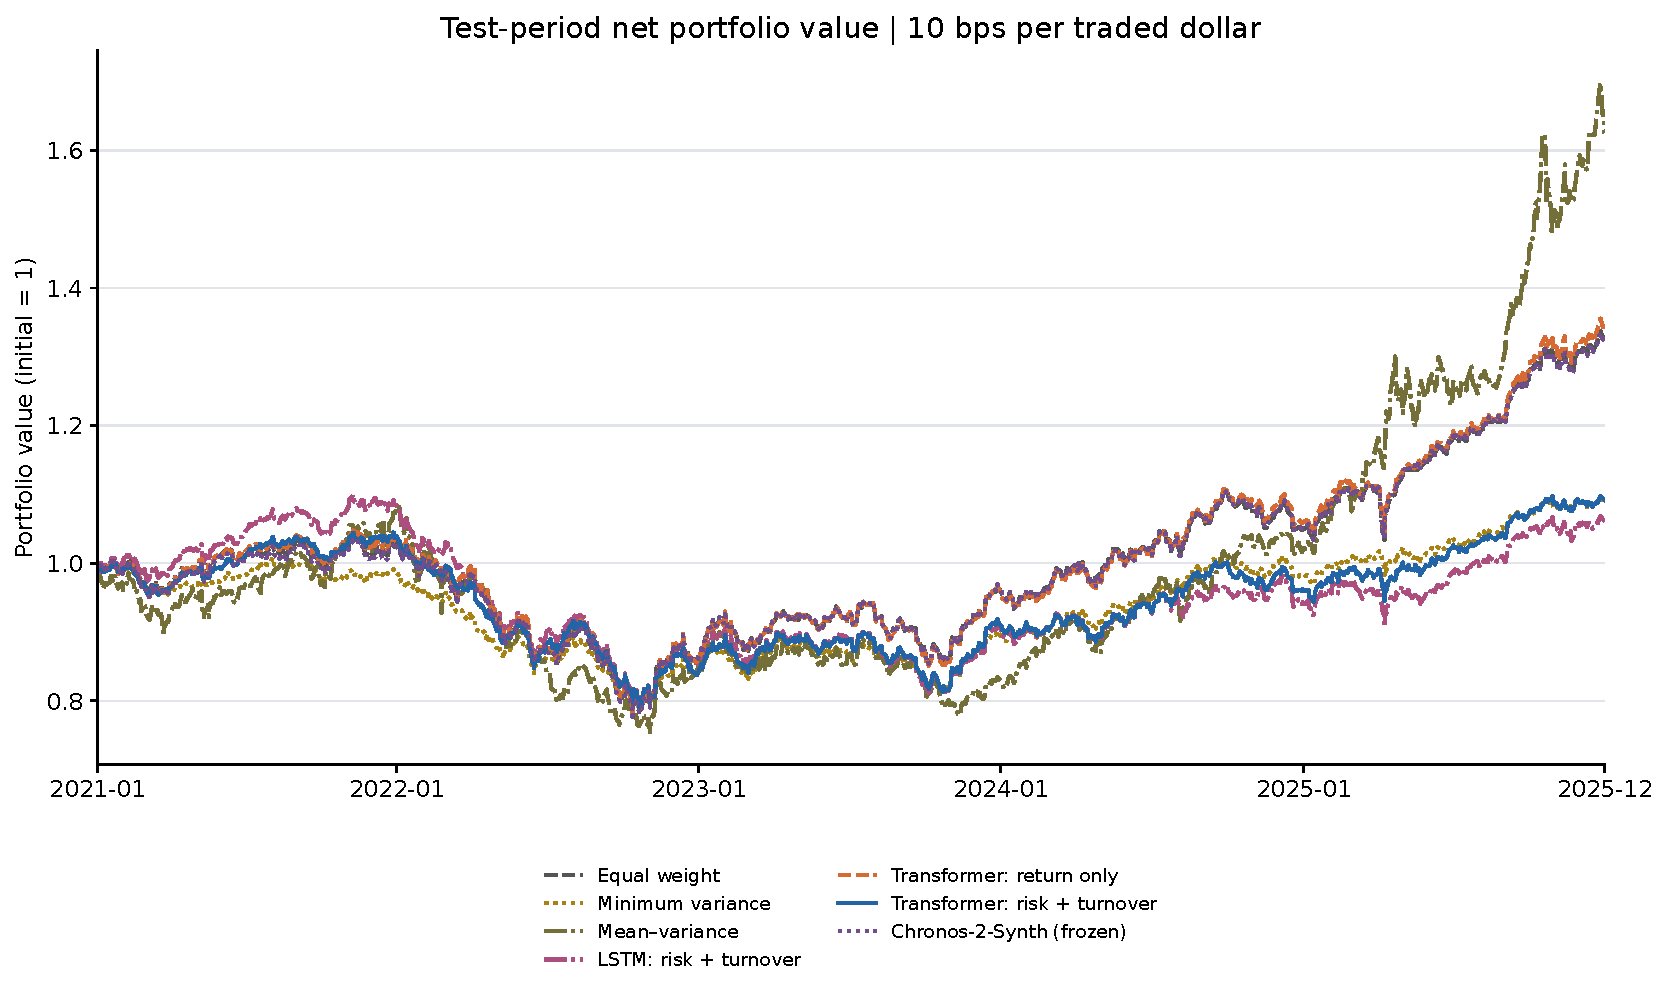
\includegraphics[width=\linewidth]{figures/cumulative_wealth.pdf}
\caption{Test-period net portfolio value at 10\,bps. The risk-penalized Transformer (blue)
tracks the bond-heavy baselines after the 2022 drawdown and misses the 2023--2025 recovery.}
\label{fig:wealth}
\end{figure}

\textbf{Failure analysis.} The risk penalty learns a low-variance, bond-heavy allocation. On
test, the full ensemble holds on average 45\% IEF and 21\% TLT, compared with 11\% and 21\%
for return-only. Rolling minimum variance (76\% IEF) behaves the same way. In the training and
validation data this was a sensible hedge: the daily SPY--IEF correlation was $-0.42$ in
2006--2017 and $-0.46$ in 2018--2020. In 2021--2025 it was $+0.07$, and in 2022 IEF and TLT fell
15\% and 31\% alongside equities. The penalty therefore fit a diversification pattern that broke
in the test period (Figure~\ref{fig:wealth}). Our validation window, which includes the 2020
crash when Treasuries hedged equities, rewarded exactly this pattern, so selecting
$\lambda_r=20$ (the edge of our grid) on validation made the problem worse.

\textbf{Costs and baselines.} The turnover penalty reduces cost drag: from 0 to 25\,bps the full
ensemble loses 0.09 Sharpe, versus 0.13 for return-only and 0.29 for risk-only. Penalizing
variance without turnover \emph{increased} trading (10.6 vs.\ 5.2), so the two penalties do not
act independently. Among baselines, mean--variance has the best test Sharpe (0.53) but the worst
validation Sharpe (0.22) and a 30\% drawdown, from concentrated SPY/GLD positions. No method ranks
consistently across the two periods. The frozen Chronos baseline stays close to equal weight in
both periods.

\textbf{Caveats.} The test set has now been evaluated once under a locked protocol. Any change
we make in response to it will be reported as post hoc rather than as an untouched test.
Penalty strengths were calibrated on one seed and one validation path, and several return-only
seeds stopped at epoch 1, so early stopping partly fits validation noise. Seed variation
measures training noise, not market uncertainty. The ETF universe is fixed in hindsight,
adjusted opens are a research proxy rather than tradable quotes, and costs are linear. Pipeline
checks pass: 53 unit tests (causality, boundary exclusion, cost accounting) and 2,931 automated
consistency checks on the saved results.

\begin{figure*}[t]
\centering
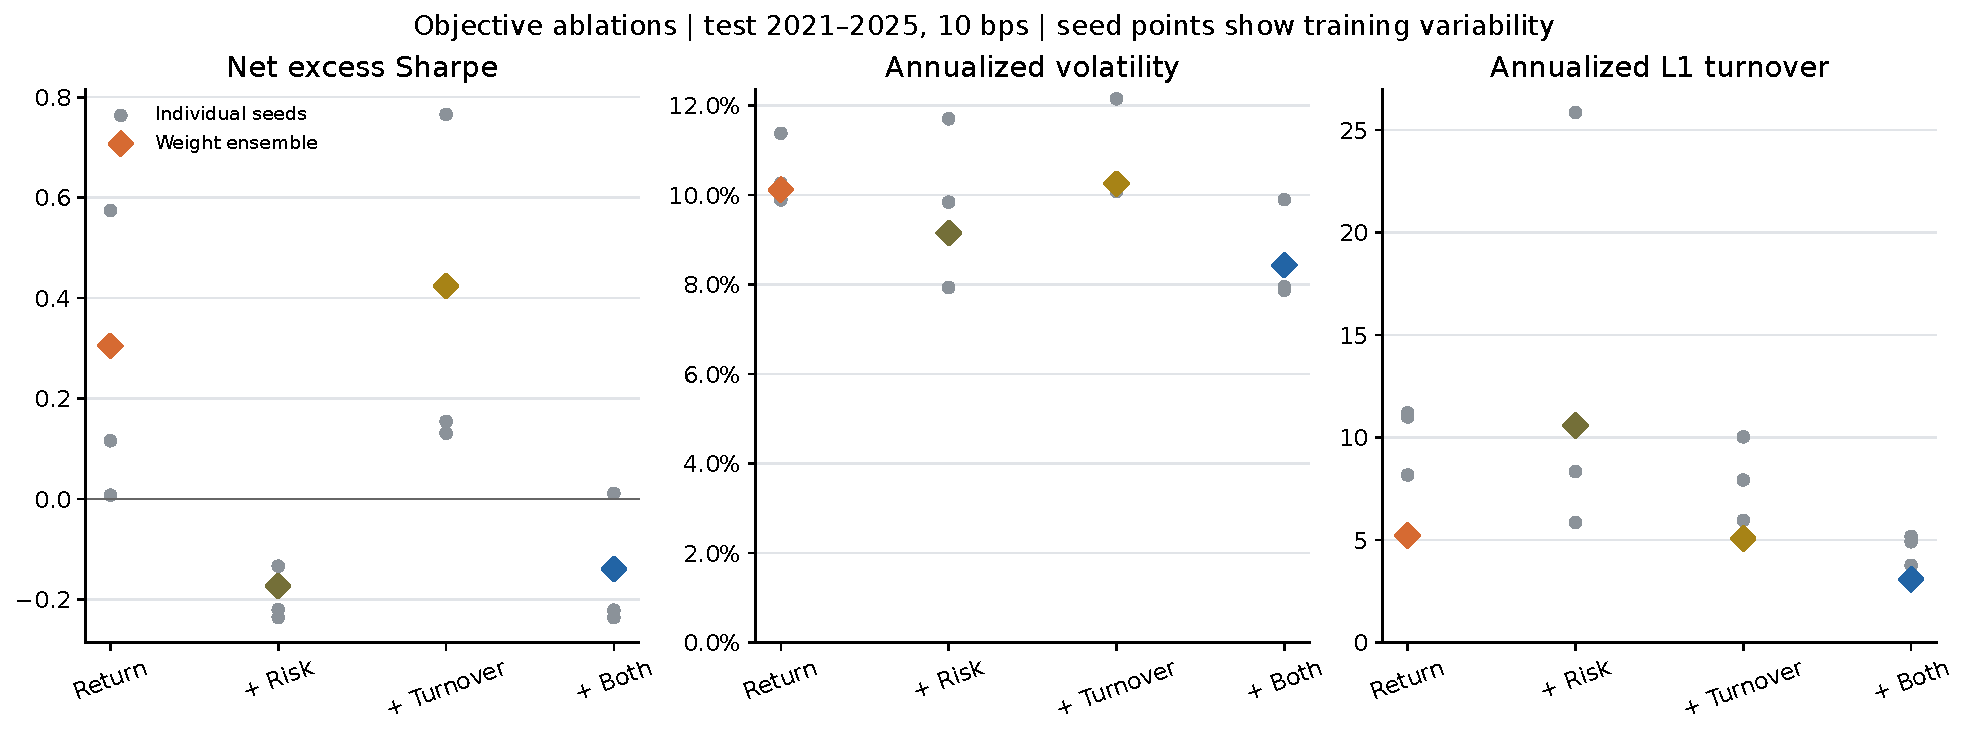
\includegraphics[width=0.92\linewidth]{figures/ablations.pdf}
\caption{Objective ablations on the test period at 10\,bps. Grey dots are individual seeds and
diamonds are weight ensembles. The penalties lower volatility and turnover as intended, but the
variance penalty lowers the Sharpe ratio.}
\label{fig:ablation}
\end{figure*}

%-------------------------------------------------------------------------
\section{Plan for the Final Report}

(1)~\textbf{Walk-forward selection.} Replace the single 2018--2020 validation window with
expanding-window refits and multiple validation folds, so that $\lambda_r$, $\lambda_t$ and
stopping are chosen across several stock--bond regimes, and widen the $\lambda_r$ grid.
(2)~\textbf{Regime analysis.} Break performance down by rolling stock--bond correlation and
volatility regime to test whether the penalty fails only when that correlation turns positive.
(3)~\textbf{Alternative risk terms.} Compare variance with downside risk (semivariance or CVaR)
and a direct Sharpe loss~\cite{zhang2020deep}, which may concentrate less on bonds.
(4)~\textbf{Consolidation.} Merge the two implementations into one reported pipeline, report
matched-budget ablations, and move the alternative implementation to a robustness appendix.
(5)~\textbf{Reporting.} Keep the current test results as the primary pre-registered outcome and
label every later change as post hoc.

{\small
\begin{thebibliography}{9}\setlength{\itemsep}{0pt}
\bibitem{zhang2020deep} Z.~Zhang, S.~Zohren, and S.~Roberts. Deep learning for portfolio
optimization. \emph{J. Financial Data Science}, 2(4):8--20, 2020.
\bibitem{kisiel2023portfolio} D.~Kisiel and D.~Gorse. Portfolio Transformer for attention-based
asset allocation. In \emph{ICAISC 2022}, LNCS 13588, Springer, 2023.
\bibitem{demiguel2009optimal} V.~DeMiguel, L.~Garlappi, and R.~Uppal. Optimal versus naive
diversification: How inefficient is the 1/N portfolio strategy? \emph{Rev. Financial Studies},
22(5):1915--1953, 2009.
\bibitem{ledoit2008robust} O.~Ledoit and M.~Wolf. Robust performance hypothesis testing with the
Sharpe ratio. \emph{J. Empirical Finance}, 15(5):850--859, 2008.
\bibitem{ansari2024chronos} A.~F.~Ansari et al. Chronos: Learning the language of time series.
\emph{TMLR}, 2024. Checkpoint used: \url{https://huggingface.co/autogluon/chronos-2-synth}.
\bibitem{yfinance} R.~Aroussi. yfinance. \url{https://github.com/ranaroussi/yfinance}.
\bibitem{deepdow} J.~Krepl. DeepDow. \url{https://github.com/jankrepl/deepdow}.
\bibitem{fred_dtb3} Board of Governors of the Federal Reserve System. 3-Month Treasury Bill
Secondary Market Rate (DTB3). FRED, Federal Reserve Bank of St. Louis.
\end{thebibliography}
}

\end{document}
